\section{Design}

In this section I begin by detailing the design for the AST to CFG conversion. I will then move on to discuss the design for actually performing branch analysis with the CFG.

\subsection{Representing the CFG}

The first step is to decide on how the control flow graph should be represented. At each vertex we need to store at least:

\begin{enumerate}
\item The type statement that the vertex represents
\item A label for the vertex
\item The list of children from this vertex
\item A unique ID for the vertex
\end{enumerate}

These may not be all that a vertex needs to store, but at this stage it is all that is required. An AST is similar to a CFG, and for that each vertex is stored as an object with references to child AST objects. From experience, this works well for the AST, and so the design will be loosely copied for the CFG. Each vertex of the CFG will be an object of type CFG, and will contain a list of children.

\subsection{The Basic Case}

It makes sense to start with the most basic EOL program and convert that into a CFG. Epsilon usefully includes a tool called AST Explorer that gives a visual representation of the AST when the class EolParserWorkbench is executed. EolParserWorkbench has a string that points to an EOL file on disk, which I have modified to point to an EOL file that I can easily modify. For a simple Hello World application, the AST explorer shown in Figure \ref{fig:ASTExplorer} is shown. 

\begin{figure}
\centering
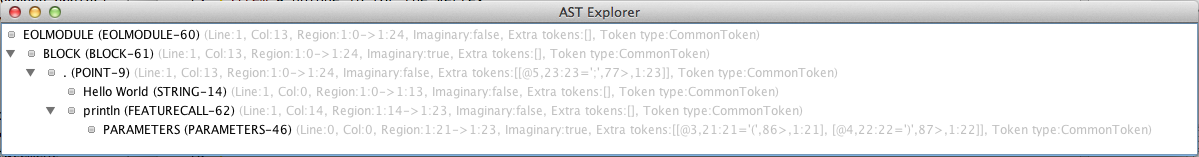
\includegraphics[width=\textwidth]{figures/ASTExplorer.png}
\caption{The AST explorer for a Hello World application}
\label{fig:ASTExplorer}
\end{figure}

The CFG for the Hello World application will have no branching points, because there are no conditional statements. The CFG for this program should look like the CFG in Figure \ref{fig:helloWorldCFG}. This looks quite similar to what happens if you perform a depth-first traversal of the AST, shown in figure \ref{fig:helloWorldDF}. Looking at the two graphs, there are differences between them. The first one is that the target CFG has a START and an END vertex. When performing the depth-first traversal, it would be simple to add a start vertex to the graph first, and link that to the root node of the AST. At each step, the last vertex found could be stored in a global variable (outside of the recursive depth-first traversal), and after the traversal has finished, the last vertex could be linked to an END vertex.

Another difference that must be addressed is that there are more vertices in the traversed AST than there are in the target CFG. This is because the AST contains all every detail of the program, so the code \verb|"Hello World".println()| is actually split into 3 vertices. The first is the string, then the point, and finally the call to the operation println. In the CFG, we are only interested in the call to the println function, the other details are not relevant to control flow. Each vertex in the AST has a type associated with it, which makes it simple to filter out types of vertices that are not relevant to the CFG. There are many different types, and so rather than blacklisting certain types, I have opted to whitelist certain types of vertices. From this hello world program, I can see that I need to add block and operation call to the whitelist.

In order to correctly join up the CFG, the use of the global variable that points to the last found AST vertex will be modified slightly. At each AST vertex, when the type is contained in the whitelist, the previously found vertex will have its child list updated to include the current vertex, and then the global pointer to the last vertex will updated to point to this vertex. This is probably easier to understand with pseudocode:

\lstinputlisting{code/ASTtoCFG_1.pseudo}

\begin{figure}
\centering
\begin{minipage}{.4\textwidth}
  \centering
    \includedot[width=0.4\linewidth]{figures/helloworld_CFG}
    \caption{The target CFG for the Hello World program}
    \label{fig:helloWorldCFG}
\end{minipage}%
\begin{minipage}{.15\textwidth}
\hspace{1cm}
\end{minipage}
\begin{minipage}{.4\textwidth}
  \centering
  \includedot[width=0.4\linewidth]{figures/helloworld2_CFG}
  \caption{The result of a depth-first traversal of the AST}
  \label{fig:helloWorldDF}
\end{minipage}
\end{figure}

At this point it hasn't been discussed how an AST object will link to a CFG object. Because the conversion code makes use of both, it needs to be easy to switch between accessing the two. One possible way of doing this is to use a hashtable with the AST vertex as a key, and a CFG object as the value. An alternative option is to modify the AST class to have an associated CFG class. Both approaches have their merits and drawbacks. The first method means that only the number of CFG objects need to be created as is absolutely necessary. However the second approach means that an AST can easily pass information into the constructor of the CFG, without it having to be dealt with by the class that is doing the conversion from AST to CFG. Because of this, I have opted to go for the latter approach, which is why in the pseudocode there is a call \verb|current.cfg| that represents getting the CFG from the AST object \verb|current|.

\subsection{Visualising the CFG}

GraphViz was introduced in the literature review, and is what will be used for turning the CFG stored in memory into a visual representation. This will make it a lot easier to test and debug the code that is doing the conversion. Similarly, while the AST explorer provides a lot of information, it is not easy to quickly visualise how the tree looks, so the AST will also be visualised using graphs drawn by GraphViz.

\subsection{The if statement}

Now that the core of the algorithm is designed, it needs to be extended to deal with statements that can send the control flow in more than one direction. I will begin by looking at the if statement, because it is one of the more simple statements.

When the depth first search reaches an if statement, it first of all needs to determine if it's an if or an if .. else statement, by looking at the number of children that it has. For the time being we assume that it has found just an if statement. The algorithm needs to add an edge from the if statement vertex to the vertex that comes after the if block. The naive approach to this would be to get the next sibling of the if statement. This doesn't work though when the if statement is the last statement within the current block. This could be fixed by looking at the parent of the sibling of the current block, but the code quickly becomes tricky to manage.

The situation is further complicated when we consider what was discussed in the analysis section about the final statement in a loop going back to the for or while loop vertex. So the problem in short then is that we don't know where the next whitelisted vertex in the AST is going to be, so we can't add an edge from the if statement to the next statement. Let's temporarily forget about this and look at the other path from the if statement - when it evaluates to true there will be some more vertices to add to our CFG. The depth-first traversal of the AST will add these correctly to the CFG. 